\documentclass[11pt,a4paper]{article}
\usepackage[utf8]{inputenc}
\usepackage[T1]{fontenc}
\usepackage{geometry}
\usepackage{xcolor}
\usepackage{tcolorbox}
\usepackage{enumitem}
\usepackage{hyperref}
\usepackage{booktabs}
\usepackage{longtable}
\usepackage{graphicx}
\usepackage{fancyhdr}
\usepackage{pgfplots}
\usepackage{tikz}
\usepackage[table]{xcolor}
\pgfplotsset{compat=1.18}

\definecolor{tablerowgray}{RGB}{245,245,245}

\geometry{margin=1in}
\setlength{\headheight}{14pt}

\definecolor{strengthgreen}{RGB}{46,125,50}
\definecolor{warningorange}{RGB}{245,124,0}
\definecolor{criticalred}{RGB}{198,40,40}
\definecolor{infocolor}{RGB}{33, 33, 33}

\pagestyle{fancy}
\fancyhf{}
\rhead{Architectural Validation Report}
\lhead{JavaBrew Platform}
\rfoot{Page \thepage}

\title{\textbf{Architectural Blueprint Validation Report}\\
\large JavaBrew Vending Machine Management Platform}
\author{Automated Traceability Analysis}
\date{\today}

\begin{document}

\maketitle

\begin{abstract}
This report validates the architectural blueprint of the JavaBrew vending machine platform through comprehensive traceability analysis. The assessment examines 51 requirements, 28 use cases, architectural components, and test coverage. The report identifies critical gaps in offline operation support, component responsibility clarity, and remote maintenance implementation, while recognizing strong fundamentals in layered architecture design and comprehensive test coverage. Actionable recommendations are provided to address identified risks before production deployment.
\end{abstract}

\tableofcontents
\newpage

\section{Executive Summary}

\subsection{Assessment Overview}

This validation analyzes the architectural blueprint using traceability extraction from project documentation. The system demonstrates strong coverage in core transaction flows but exhibits critical gaps in operational resilience and edge case handling.

\subsubsection{Coverage Metrics}

Table~\ref{tab:metrics-summary} provides high-level project metrics. Figures~\ref{fig:coverage-metrics}, \ref{fig:test-distribution}, and \ref{fig:risk-distribution} visualize the coverage distribution, test pyramid, and risk severity.

\begin{table}[h]
\centering
\begin{tabular}{@{}lrrr@{}}
\toprule
\textbf{Metric Category} & \textbf{Total} & \textbf{Covered} & \textbf{Coverage} \\
\midrule
Requirements & 51 & 38 & 74.5\% \\
Use Cases & 28 & 26 & 92.9\% \\
Tests & 158 & 158 & 100\% \\
Architecture Layers & 6 & 6 & 100\% \\
Critical Risks & 3 & --- & 3 Critical \\
\bottomrule
\end{tabular}
\caption{Project Metrics Summary}
\label{tab:metrics-summary}
\end{table}

\begin{figure}[h]
\centering
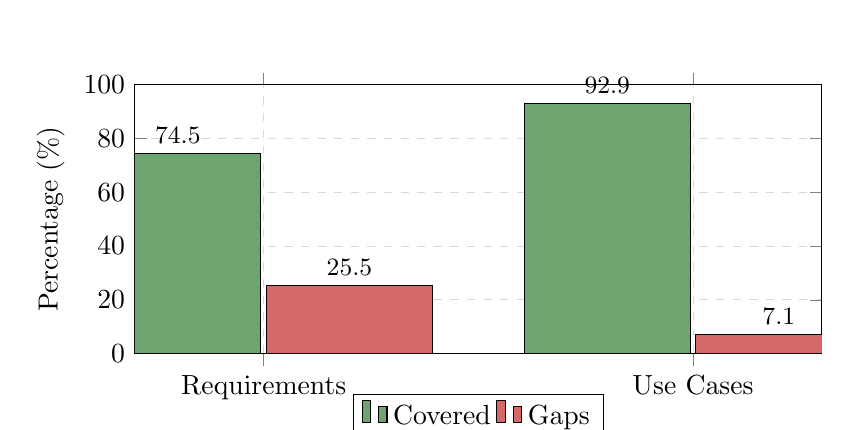
\begin{tikzpicture}
\begin{axis}[
    ybar,
    width=0.85\textwidth,
    height=5cm,
    ylabel={Percentage (\%)},
    symbolic x coords={Requirements, Use Cases},
    xtick=data,
    ymin=0, ymax=100,
    bar width=60pt,
    enlarge x limits=0.3,
    legend style={at={(0.5,-0.15)}, anchor=north, legend columns=-1},
    nodes near coords,
    nodes near coords style={font=\small},
    grid=major,
    grid style={dashed,gray!30}
]
\addplot[fill=strengthgreen!70] coordinates {(Requirements,74.5) (Use Cases,92.9)};
\addplot[fill=criticalred!70] coordinates {(Requirements,25.5) (Use Cases,7.1)};
\legend{Covered, Gaps}
\end{axis}
\end{tikzpicture}
\caption{Requirements and Use Case Coverage}
\label{fig:coverage-metrics}
\end{figure}

\begin{figure}[h]
\centering
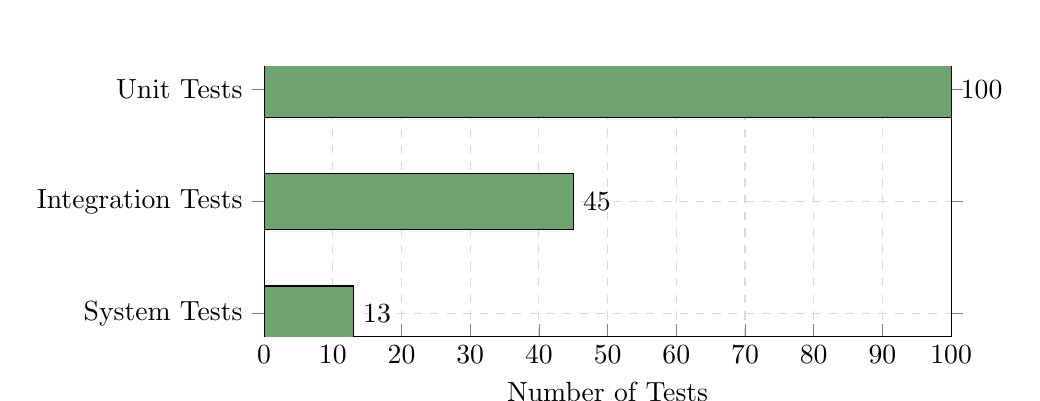
\begin{tikzpicture}
\begin{axis}[
    xbar,
    width=0.85\textwidth,
    height=5cm,
    xlabel={Number of Tests},
    symbolic y coords={System Tests, Integration Tests, Unit Tests},
    ytick=data,
    xmin=0, xmax=100,
    bar width=20pt,
    nodes near coords,
    nodes near coords align={horizontal},
    grid=major,
    grid style={dashed,gray!30}
]
\addplot[fill=strengthgreen!70] coordinates {(100,{Unit Tests}) (45,{Integration Tests}) (13,{System Tests})};
\end{axis}
\end{tikzpicture}
\caption{Test Distribution: 158 Total Tests (Unit 63\%, Integration 29\%, System 8\%)}
\label{fig:test-distribution}
\end{figure}

\begin{figure}[h]
\centering
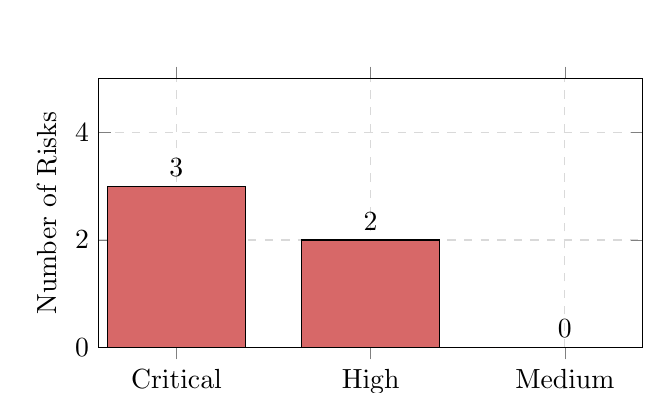
\begin{tikzpicture}
\begin{axis}[
    ybar,
    width=0.7\textwidth,
    height=5cm,
    ylabel={Number of Risks},
    symbolic x coords={Critical, High, Medium},
    xtick=data,
    ymin=0, ymax=5,
    bar width=50pt,
    enlarge x limits=0.2,
    nodes near coords,
    nodes near coords style={font=\normalsize},
    grid=major,
    grid style={dashed,gray!30}
]
\addplot[fill=criticalred!70] coordinates {(Critical,3) (High,2) (Medium,0)};
\end{axis}
\end{tikzpicture}
\caption{Risk Distribution by Severity}
\label{fig:risk-distribution}
\end{figure}

\subsection{Critical Findings}

\begin{tcolorbox}[colback=criticalred!5,colframe=criticalred,title=\textbf{Critical Issues Requiring Immediate Attention}]
\begin{enumerate}
    \item \textbf{Offline Operation Unsupported:} Three requirements for disconnected vending machine operation are completely unimplemented, creating a single point of failure on network connectivity that makes the system non-operational during outages.

    \item \textbf{Vague Component Responsibilities:} Multiple architectural components lack precise responsibility definitions, violating the Single Responsibility Principle and risking architectural degradation as complexity increases.

    \item \textbf{Remote Maintenance Partially Implemented:} Backend task tracking exists but the hardware abstraction layer for sending commands to physical devices is absent, making promised remote control features undeliverable.
\end{enumerate}
\end{tcolorbox}

\begin{tcolorbox}[colback=strengthgreen!5,colframe=strengthgreen,title=\textbf{Architectural Strengths}]
\begin{itemize}[leftmargin=*]
    \item Well-structured layered architecture with clean separation of concerns
    \item Comprehensive test coverage with 158 tests following the test pyramid principle
    \item Effective design patterns (Builder, DAO, Mapper) applied judiciously
    \item Complete traceability from requirements through use cases to tests
    \item Dual database strategy (H2 for tests, PostgreSQL for production) enabling fast feedback loops
    \item Extensive error path testing for robustness and graceful degradation
\end{itemize}
\end{tcolorbox}

\newpage

\section{Project Inventory}

\subsection{Requirements Inventory}

\rowcolors{2}{white}{tablerowgray}
\begin{longtable}{@{}p{0.08\textwidth}p{0.50\textwidth}p{0.12\textwidth}@{}}
\caption{Complete Requirements List} \label{tab:all-requirements} \\
\toprule
\rowcolor{white}\textbf{ID} & \textbf{Requirement Description} & \textbf{Status} \\
\midrule
\endfirsthead
\multicolumn{3}{c}{{\tablename\ \thetable{} -- continued from previous page}} \\
\toprule
\rowcolor{white}\textbf{ID} & \textbf{Requirement Description} & \textbf{Status} \\
\midrule
\endhead
\midrule
\multicolumn{3}{r}{{Continued on next page}} \\
\endfoot
\bottomrule
\endlastfoot

\label{req:1}\hyperref[req:1]{REQ-1} & Modernize product management through vending machines & Unsupported \\
\label{req:2}\hyperref[req:2]{REQ-2} & Integrated, simple, secure platform for all users & Unsupported \\
\label{req:3}\hyperref[req:3]{REQ-3} & QR code scanning for product purchase & Covered \\
\label{req:4}\hyperref[req:4]{REQ-4} & Dashboard with sales and malfunction statistics & Covered \\
\label{req:5}\hyperref[req:5]{REQ-5} & Monitor sales and stock levels & Covered \\
\label{req:6}\hyperref[req:6]{REQ-6} & Improve user experience and reduce operator response time & Unsupported \\
\label{req:7}\hyperref[req:7]{REQ-7} & Scalable service aligned with modern technologies & Unsupported \\
\label{req:8}\hyperref[req:8]{REQ-8} & Real-time inventory tracking & Covered \\
\label{req:9}\hyperref[req:9]{REQ-9} & Support digital payment methods & Covered \\
\label{req:10}\hyperref[req:10]{REQ-10} & Centralized management tool for maintenance & Covered \\
\label{req:11}\hyperref[req:11]{REQ-11} & Integrate digital payments and remote monitoring & Covered \\
\label{req:12}\hyperref[req:12]{REQ-12} & Improve machine management & Unsupported \\
\label{req:13}\hyperref[req:13]{REQ-13} & User registration and wallet balance viewing & Covered \\
\label{req:14}\hyperref[req:14]{REQ-14} & Account recharge with cash or online methods & Covered \\
\label{req:15}\hyperref[req:15]{REQ-15} & Automatic balance deduction from wallet & Covered \\
\label{req:16}\hyperref[req:16]{REQ-16} & Admin interface for machine configuration and pricing & Covered \\
\label{req:17}\hyperref[req:17]{REQ-17} & CRUD operations for users, machines, items & Covered \\
\label{req:18}\hyperref[req:18]{REQ-18} & Automated reporting for maintenance technicians & Covered \\
\label{req:19}\hyperref[req:19]{REQ-19} & Detect disconnected vending machines & \textcolor{criticalred}{Unsupported} \\
\label{req:20}\hyperref[req:20]{REQ-20} & Offline register for local transaction tracking & \textcolor{criticalred}{Unsupported} \\
\label{req:21}\hyperref[req:21]{REQ-21} & Synchronize local transactions with central database & \textcolor{criticalred}{Unsupported} \\
\label{req:22}\hyperref[req:22]{REQ-22} & Allow anonymous cash transactions & Covered \\
\label{req:23}\hyperref[req:23]{REQ-23} & Strategic product selection for cost minimization & Unsupported \\
\label{req:24}\hyperref[req:24]{REQ-24} & Fast maintenance to reduce investment costs & Unsupported \\
\label{req:25}\hyperref[req:25]{REQ-25} & User login with email and password & Covered \\
\label{req:26}\hyperref[req:26]{REQ-26} & Verify user credentials & Covered \\
\label{req:27}\hyperref[req:27]{REQ-27} & Provide personalized interface after authentication & Covered \\
\label{req:28}\hyperref[req:28]{REQ-28} & Display error message for incorrect credentials & Covered \\
\label{req:29}\hyperref[req:29]{REQ-29} & Admin worker management CRUD & Covered \\
\label{req:30}\hyperref[req:30]{REQ-30} & Admin task assignment mechanism & Covered \\
\label{req:31}\hyperref[req:31]{REQ-31} & Admin authentication requirement & Covered \\
\label{req:32}\hyperref[req:32]{REQ-32} & Display user and item analytics & Covered \\
\label{req:33}\hyperref[req:33]{REQ-33} & Handle analytics loading errors & Unsupported \\
\label{req:34}\hyperref[req:34]{REQ-34} & Allow admin to create new vending machine & Covered \\
\label{req:35}\hyperref[req:35]{REQ-35} & Verify machine creation data & Covered \\
\label{req:36}\hyperref[req:36]{REQ-36} & Save machine to database & Covered \\
\label{req:37}\hyperref[req:37]{REQ-37} & Error handling for missing fields & Covered \\
\label{req:38}\hyperref[req:38]{REQ-38} & Error message for save failure & Covered \\
\label{req:39}\hyperref[req:39]{REQ-39} & Support three user types: admin, worker, customer & Covered \\
\label{req:40}\hyperref[req:40]{REQ-40} & Admin full application access & Covered \\
\label{req:41}\hyperref[req:41]{REQ-41} & Worker maintenance and assistance operations & Covered \\
\label{req:42}\hyperref[req:42]{REQ-42} & Customer machine interaction for purchases & Covered \\
\label{req:43}\hyperref[req:43]{REQ-43} & User table with common attributes & Unsupported \\
\label{req:44}\hyperref[req:44]{REQ-44} & Role-specific table extensions & Unsupported \\
\label{req:45}\hyperref[req:45]{REQ-45} & Efficient user login management & Unsupported \\
\label{req:46}\hyperref[req:46]{REQ-46} & Transaction data management & Unsupported \\
\label{req:47}\hyperref[req:47]{REQ-47} & Transaction item details table & Unsupported \\
\label{req:48}\hyperref[req:48]{REQ-48} & Maintain transaction-item relationships & Unsupported \\
\label{req:49}\hyperref[req:49]{REQ-49} & Track active user-machine connections & Covered \\
\label{req:50}\hyperref[req:50]{REQ-50} & Facilitate user-concrete machine communication & Unsupported \\
\label{req:51}\hyperref[req:51]{REQ-51} & Enable future remote maintenance development & Partially \\
\end{longtable}

\subsection{Use Cases Inventory}

\rowcolors{2}{white}{tablerowgray}
\begin{longtable}{@{}p{0.08\textwidth}p{0.35\textwidth}p{0.12\textwidth}p{0.15\textwidth}@{}}
\caption{Complete Use Cases List} \label{tab:all-usecases} \\
\toprule
\rowcolor{white}\textbf{ID} & \textbf{Use Case Name} & \textbf{Actor} & \textbf{Status} \\
\midrule
\endfirsthead
\multicolumn{4}{c}{{\tablename\ \thetable{} -- continued from previous page}} \\
\toprule
\rowcolor{white}\textbf{ID} & \textbf{Use Case Name} & \textbf{Actor} & \textbf{Status} \\
\midrule
\endhead
\midrule
\multicolumn{4}{r}{{Continued on next page}} \\
\endfoot
\bottomrule
\endlastfoot

\label{uc:1}\hyperref[uc:1]{UC-1} & Purchase Product via QR Code & User & Covered \\
\label{uc:2}\hyperref[uc:2]{UC-2} & Monitor Sales and Malfunctions & Admin & Covered \\
\label{uc:3}\hyperref[uc:3]{UC-3} & Plan Maintenance and Restocking & Admin & Covered \\
\label{uc:4}\hyperref[uc:4]{UC-4} & User Registration and Login & Customer & Covered \\
\label{uc:5}\hyperref[uc:5]{UC-5} & Wallet Reloading & Customer & Covered \\
\label{uc:6}\hyperref[uc:6]{UC-6} & Admin Management & Admin & Covered \\
\label{uc:7}\hyperref[uc:7]{UC-7} & Maintenance and Refilling & Worker & Covered \\
\label{uc:8}\hyperref[uc:8]{UC-8} & Use Case Template Description & --- & Template \\
\label{uc:9}\hyperref[uc:9]{UC-9} & User Login & User & Covered \\
\label{uc:10}\hyperref[uc:10]{UC-10} & User Sign up & User & Covered \\
\label{uc:11}\hyperref[uc:11]{UC-11} & User Login (Detailed) & User & Covered \\
\label{uc:12}\hyperref[uc:12]{UC-12} & Buy item & Customer & Covered \\
\label{uc:13}\hyperref[uc:13]{UC-13} & Recharge account & Customer & Covered \\
\label{uc:14}\hyperref[uc:14]{UC-14} & Connect to Vending Machine & Customer & Covered \\
\label{uc:15}\hyperref[uc:15]{UC-15} & Buy Item (Detailed) & Customer & Covered \\
\label{uc:16}\hyperref[uc:16]{UC-16} & Recharge Balance (Detailed) & Customer & Covered \\
\label{uc:17}\hyperref[uc:17]{UC-17} & View task details & Worker & Covered \\
\label{uc:18}\hyperref[uc:18]{UC-18} & Mark task as completed & Worker & Covered \\
\label{uc:19}\hyperref[uc:19]{UC-19} & Mark task as completed (Detailed) & Worker & Covered \\
\label{uc:20}\hyperref[uc:20]{UC-20} & View Analytics & Admin & Covered \\
\label{uc:21}\hyperref[uc:21]{UC-21} & Manage Workers CRUD & Admin & Covered \\
\label{uc:22}\hyperref[uc:22]{UC-22} & Manage Vending Machines CRUD & Admin & Covered \\
\label{uc:23}\hyperref[uc:23]{UC-23} & Assign Task & Admin & Covered \\
\label{uc:24}\hyperref[uc:24]{UC-24} & View Workers & Admin & Covered \\
\label{uc:25}\hyperref[uc:25]{UC-25} & View Tasks & Admin & Covered \\
\label{uc:26}\hyperref[uc:26]{UC-26} & Create New Vending Machine & Admin & Covered \\
\label{uc:27}\hyperref[uc:27]{UC-27} & Track Active Connections & User, Machine & Covered \\
\label{uc:28}\hyperref[uc:28]{UC-28} & Remote Maintenance Management & Technician, Admin & \textcolor{warningorange}{Partial} \\
\end{longtable}

\subsection{Test Suite Inventory}

\rowcolors{2}{white}{tablerowgray}
\begin{longtable}{@{}p{0.06\textwidth}p{0.48\textwidth}p{0.10\textwidth}@{}}
\caption{Test Suite Overview (158 Tests Total)} \label{tab:all-tests} \\
\toprule
\rowcolor{white}\textbf{Type} & \textbf{Coverage Area} & \textbf{Count} \\
\midrule
\endfirsthead
\multicolumn{3}{c}{{\tablename\ \thetable{} -- continued from previous page}} \\
\toprule
\rowcolor{white}\textbf{Type} & \textbf{Coverage Area} & \textbf{Count} \\
\midrule
\endhead
\midrule
\multicolumn{3}{r}{{Continued on next page}} \\
\endfoot
\bottomrule
\endlastfoot

\label{test:unit}\hyperref[test:unit]{Unit} & Login/Registration validation, service logic isolation & 100 \\
\label{test:integration}\hyperref[test:integration]{Integration} & DAO operations, service-database interaction, CRUD flows & 45 \\
\label{test:system}\hyperref[test:system]{System} & End-to-end use case validation, error handling workflows & 13 \\
\end{longtable}

\section{Requirements Coverage Analysis}

\subsection{Offline Operation: Critical Gap}

The most significant coverage gap involves offline operation during network outages. Three requirements explicitly specify behavior when vending machines lose connectivity:

\begin{tcolorbox}[colback=criticalred!5,colframe=criticalred,title=\textbf{Unsupported Offline Requirements}]
\hyperref[req:19]{REQ-19} - \textbf{Detect Disconnected Machines:} System must implement polling to detect when vending machines lose Internet connectivity.

\hyperref[req:20]{REQ-20} - \textbf{Offline Transaction Register:} System must maintain local storage on machines to track transactions during disconnection periods.

\hyperref[req:21]{REQ-21} - \textbf{Synchronization Protocol:} Once connectivity is restored, locally stored transactions must synchronize with the central database.
\end{tcolorbox}

\textbf{Architectural Impact:} The current architecture assumes persistent connectivity throughout transaction flows. No components exist for:
\begin{itemize}
    \item Local transaction storage on vending machine firmware
    \item Connection state monitoring and detection
    \item Conflict resolution or eventual consistency protocols
    \item Offline authentication or authorization fallbacks
\end{itemize}

Without offline capabilities, machines become completely non-operational during any network disruption, directly impacting revenue and customer experience. This represents a fundamental architectural assumption that may not hold in real-world deployments.

\subsection{Requirements Quality Issues}

Table~\ref{tab:vague-requirements} identifies requirements with insufficient specificity and their architectural impact.

\rowcolors{2}{white}{tablerowgray}
\begin{longtable}{@{}p{0.12\textwidth}p{0.35\textwidth}p{0.40\textwidth}@{}}
\caption{Vague Requirements Impacting Design} \label{tab:vague-requirements} \\
\toprule
\rowcolor{white}\textbf{Req ID} & \textbf{Issue} & \textbf{Architectural Impact} \\
\midrule
\endfirsthead
\multicolumn{3}{c}{{\tablename\ \thetable{} -- continued from previous page}} \\
\toprule
\rowcolor{white}\textbf{Req ID} & \textbf{Issue} & \textbf{Architectural Impact} \\
\midrule
\endhead
\midrule
\multicolumn{3}{r}{{Continued on next page}} \\
\endfoot
\bottomrule
\endlastfoot

\label{req:2}\hyperref[req:2]{REQ-2} & Security attributes undefined & Cannot design threat model or security architecture without knowing which attack vectors matter \\
\label{req:6}\hyperref[req:6]{REQ-6} & UX improvements lack metrics & Impossible to validate if architecture achieves goals without quantifiable targets \\
\label{req:7}\hyperref[req:7]{REQ-7} & Scalability criteria unspecified & Cannot determine if design supports required throughput, concurrent users, or data volume \\
\label{req:12}\hyperref[req:12]{REQ-12} & Management improvement undefined & Lacks specific business metrics to measure architecture success \\
\label{req:33}\hyperref[req:33]{REQ-33} & Error handling scope unclear & May result in inconsistent error responses without standardized format \\
\label{req:51}\hyperref[req:51]{REQ-51} & Remote maintenance scope vague & Unclear what hardware control functions are required for implementation \\
\end{longtable}

\section{Use Case Analysis}

\subsection{Use Case Coverage Status}

The majority of use cases (26 of 28, or 92.9\%) have associated requirements and architectural components. Table~\ref{tab:uc-status} provides a summary of coverage status.

\begin{table}[h]
\centering
\begin{tabular}{@{}lrr@{}}
\toprule
\textbf{Status} & \textbf{Count} & \textbf{Percentage} \\
\midrule
Fully Covered & 24 & 85.7\% \\
Partially Covered & 2 & 7.1\% \\
Not Covered & 2 & 7.1\% \\
\bottomrule
\end{tabular}
\caption{Use Case Coverage Distribution}
\label{tab:uc-status}
\end{table}

\subsection{Partially Covered Use Cases}

\begin{tcolorbox}[colback=warningorange!5,colframe=warningorange,title=\textbf{Use Cases Requiring Attention}]
\hyperref[uc:28]{UC-28} - \textbf{Remote Maintenance Management:} Backend task tracking services exist, but the hardware abstraction layer for sending commands to physical devices is absent. The promise of remote control capabilities (unlocking jammed products, diagnostics) cannot be fulfilled without device gateway components.

\hyperref[uc:8]{UC-8} - \textbf{Use Case Template Description:} This use case serves as documentation template rather than functional requirement. Contains no actor, flow, or test specifications. Adds no value to traceability.
\end{tcolorbox}

\section{Architectural Quality Assessment}

\subsection{Layered Architecture Structure}

The architecture implements a six-layer pattern with clear separation of concerns. Table~\ref{tab:architecture-layers} details each layer's responsibilities.

\begin{table}[h]
\centering
\begin{tabular}{@{}p{0.20\textwidth}p{0.35\textwidth}p{0.35\textwidth}@{}}
\toprule
\textbf{Layer} & \textbf{Responsibility} & \textbf{Key Components} \\
\midrule
Presentation & UI/UX and user interaction & Mockups, web interfaces, mobile app \\
\midrule
Controllers & HTTP routing and input validation & UserController, AdminController, CustomerController \\
\midrule
Services & Business logic orchestration & UserService, AdminService, CustomerService \\
\midrule
DAO & Data access abstraction & UserDao, TransactionDao, ItemDao, MachineDao \\
\midrule
ORM & Object-relational mapping & Hibernate, JPA annotations \\
\midrule
Database & Data persistence & PostgreSQL (production), H2 (testing) \\
\bottomrule
\end{tabular}
\caption{Six-Layer Architecture}
\label{tab:architecture-layers}
\end{table}

\textbf{Layering Benefits:} Dependencies flow strictly downward; controllers delegate to services; services call DAOs. This structure enables independent layer testing, technology substitution, and clear responsibility boundaries.

\subsection{Component Responsibility Issues}

\begin{tcolorbox}[colback=criticalred!5,colframe=criticalred,title=\textbf{Single Responsibility Principle Violations}]
\textbf{Services Layer:} Described as "contains business logic" without specifying bounded contexts. Risk of accumulating responsibilities across customer purchases, admin configuration, worker maintenance, and user management in a monolithic service layer.

\textbf{DAO Layer:} "Manages data access and retrieval" is too generic. Without specific DAO responsibilities (UserDao handles user CRUD only, TransactionDao handles financial records only), risk of sprawling DAO classes.

\textbf{Database Component:} Overlaps with DAO responsibilities. Distinction between DBManager (connection pooling), DAO classes (query execution), and ORM layer (object mapping) is unclear.
\end{tcolorbox}

\subsection{Design Patterns Application}

\begin{table}[h]
\centering
\begin{tabular}{@{}p{0.18\textwidth}p{0.32\textwidth}p{0.40\textwidth}@{}}
\toprule
\textbf{Pattern} & \textbf{Application} & \textbf{Benefit} \\
\midrule
Builder & ConcreteVendingMachine construction & Handles optional parameters; enforces required fields \\
\midrule
DAO & UserDao, TransactionDao, ItemDao, MachineDao & Abstracts persistence; enables ORM swapping \\
\midrule
Mapper & TaskMapper, ConnectionMapper, InventoryMapper & Separates domain from persistence models \\
\bottomrule
\end{tabular}
\caption{Design Patterns}
\label{tab:design-patterns}
\end{table}

Pattern application is judicious—Builder only for complex objects, DAOs for all persistent entities, Mappers for domain-database separation. No overengineering observed.

\section{Test Strategy Assessment}

\subsection{Test Infrastructure}

The testing stack demonstrates maturity:

\begin{table}[h]
\centering
\begin{tabular}{@{}p{0.25\textwidth}p{0.20\textwidth}p{0.42\textwidth}@{}}
\toprule
\textbf{Component} & \textbf{Version} & \textbf{Purpose} \\
\midrule
JUnit & 5.11.0 & Unit test execution framework \\
Mockito & 5.18.0 & Dependency isolation and mocking \\
JaCoCo & Latest & Code coverage measurement \\
H2 Database & In-memory & Fast integration test feedback \\
PostgreSQL & 16 & Production database parity \\
\bottomrule
\end{tabular}
\caption{Test Infrastructure}
\label{tab:test-infrastructure}
\end{table}

\subsection{Test Distribution}

The test pyramid is properly shaped with majority at unit level for fast feedback, integration tests validating component interaction, and system tests confirming end-to-end flows.

\subsection{Test Coverage Strengths}

\textbf{Error Path Testing:} Most use cases test multiple failure scenarios (insufficient balance, out of stock, connection errors, not found conditions), ensuring graceful degradation and robust error handling.

\textbf{DAO Layer Coverage:} Each DAO has dedicated CRUD tests verifying persistence operations, with integration tests confirming service-DAO-database interaction.

\textbf{Service Isolation:} Mockito enables service layer testing without database dependencies, providing fast feedback and deterministic test execution.

\subsection{Testing Gaps}

\rowcolors{2}{white}{tablerowgray}
\begin{longtable}{@{}p{0.20\textwidth}p{0.35\textwidth}p{0.32\textwidth}@{}}
\caption{Critical Testing Gaps} \label{tab:testing-gaps} \\
\toprule
\rowcolor{white}\textbf{Gap Type} & \textbf{Missing Coverage} & \textbf{Risk/Impact} \\
\midrule
\endfirsthead
\multicolumn{3}{c}{{\tablename\ \thetable{} -- continued from previous page}} \\
\toprule
\rowcolor{white}\textbf{Gap Type} & \textbf{Missing Coverage} & \textbf{Risk/Impact} \\
\midrule
\endhead
\midrule
\multicolumn{3}{r}{{Continued on next page}} \\
\endfoot
\bottomrule
\endlastfoot

Navigation Tests & No UI flow validation for role-based routing & Navigation bugs reach production \\
Hardware Integration & No device communication tests & Remote maintenance unverifiable \\
Performance Tests & No load/stress/concurrency tests & Scalability limits unknown \\
Security Tests & No SQL injection, auth bypass, or authorization tests & Vulnerabilities undetected \\
End-to-End Journeys & No multi-use-case sequences & Complete workflows unvalidated \\
Offline Scenarios & No disconnection/synchronization tests & Offline operation unverifiable \\
\end{longtable}

\section{PDF Documentation Validation}

\subsection{Documentation Completeness Assessment}

The PDF documentation validation achieved \textbf{68.75\% feature coverage} against a 0.85 (85\%) threshold, indicating incomplete documentation of system features and design decisions.

\begin{table}[h]
\centering
\begin{tabular}{@{}lr@{}}
\toprule
\textbf{Metric} & \textbf{Value} \\
\midrule
Coverage Percentage & 68.75\% \\
Threshold Required & 85.0\% \\
Coverage Status & \textcolor{warningorange}{Below Threshold} \\
\midrule
Total Expected Features & 16 \\
Features Found & 11 \\
Features Missing & 5 \\
\bottomrule
\end{tabular}
\caption{Documentation Validation Results}
\label{tab:doc-validation}
\end{table}

\subsection{Well-Documented Features}

\rowcolors{2}{white}{tablerowgray}
\begin{longtable}{@{}p{0.25\textwidth}p{0.12\textwidth}p{0.50\textwidth}@{}}
\caption{Well-Documented Features (High Similarity Scores)} \label{tab:documented-features} \\
\toprule
\rowcolor{white}\textbf{Feature} & \textbf{Similarity} & \textbf{Evidence} \\
\midrule
\endfirsthead
\multicolumn{3}{c}{{\tablename\ \thetable{} -- continued from previous page}} \\
\toprule
\rowcolor{white}\textbf{Feature} & \textbf{Similarity} & \textbf{Evidence} \\
\midrule
\endhead
\midrule
\multicolumn{3}{r}{{Continued on next page}} \\
\endfoot
\bottomrule
\endlastfoot

User-Centric Design & 92.7\% & Detailed mockups (Fig. 10) showing interactive product catalog with quantity controls \\
Testing Strategy & 91.2\% & Comprehensive description of unit and integration testing approach with tool configuration \\
Standardized Use Cases & 91.9\% & Documented use case template with ID, name, actors, flows, and test linkage \\
Defined Pre/Post Conditions & 91.9\% & Use case specifications include clear state conditions before and after execution \\
Layered Architecture & 90.1\% & UML component diagram (Fig. 11) showing six-layer structure with relationships \\
Role-Based Access Control & 88.9\% & Clear definition of three user types (admin, worker, customer) with table inheritance \\
Design Patterns & 90.1\% & Data Mapper pattern documented for mapper classes separating domain from persistence \\
Error Handling Process & 85.4\% & Alternative flows document error scenarios with user-facing messages \\
Database Design & 86.1\% & PostgreSQL 16 specified as production database with relational model \\
Effective Tool Utilization & 88.3\% & AI tools documented (GitHub Copilot, GPT-4.1, Claude, Gemini) with supervision notes \\
Comprehensive Test Coverage & 85.8\% & Test cases listed for each use case with numbers and verification descriptions \\
\end{longtable}

\subsection{Undocumented/Poorly-Documented Features}

Five expected features have insufficient or missing documentation:

\begin{tcolorbox}[colback=warningorange!5,colframe=warningorange,title=\textbf{Documentation Gaps}]
\begin{enumerate}
    \item \textbf{Performance Optimization Strategies:} No documentation of caching, database indexing, or query optimization approaches.
    
    \item \textbf{Security Architecture:} Authentication/authorization mechanisms described but encryption, token management, and threat model absent.
    
    \item \textbf{API Documentation:} No OpenAPI/Swagger specifications or endpoint documentation provided.
    
    \item \textbf{Deployment Architecture:} Infrastructure, containerization, scaling strategies, and monitoring not documented.
    
    \item \textbf{Data Migration Strategy:} No documentation of how existing vending machine data integrates or migrates to new system.
\end{enumerate}
\end{tcolorbox}

\textbf{Documentation Quality Assessment:} While core functional design is well-documented through use cases, mockups, and architecture diagrams, operational and infrastructure aspects lack coverage. This creates implementation ambiguity for deployment, scaling, and security hardening phases.

\section{Critical Risks and Recommendations}

\subsection{Risk Summary}

\rowcolors{2}{white}{tablerowgray}
\begin{longtable}{@{}p{0.10\textwidth}p{0.38\textwidth}p{0.12\textwidth}p{0.27\textwidth}@{}}
\caption{Critical Risks Summary} \label{tab:risk-summary} \\
\toprule
\rowcolor{white}\textbf{Risk ID} & \textbf{Risk Name} & \textbf{Severity} & \textbf{Affected Items} \\
\midrule
\endfirsthead
\multicolumn{4}{c}{{\tablename\ \thetable{} -- continued from previous page}} \\
\toprule
\rowcolor{white}\textbf{Risk ID} & \textbf{Risk Name} & \textbf{Severity} & \textbf{Affected Items} \\
\midrule
\endhead
\midrule
\multicolumn{4}{r}{{Continued on next page}} \\
\endfoot
\bottomrule
\endlastfoot

\label{risk:1}RISK-1 & Offline Operation Unavailability & \textcolor{criticalred}{Critical} & \hyperref[req:19]{REQ-19}, \hyperref[req:20]{REQ-20}, \hyperref[req:21]{REQ-21} \\
\label{risk:2}RISK-2 & Component Responsibility Ambiguity & \textcolor{criticalred}{Critical} & Services, DAO, Database layers \\
\label{risk:3}RISK-3 & Remote Maintenance Unimplementable & \textcolor{criticalred}{Critical} & \hyperref[uc:28]{UC-28}, \hyperref[req:51]{REQ-51} \\
\label{risk:4}RISK-4 & Insufficient Documentation & \textcolor{warningorange}{High} & Deployment, Security, API specs \\
\label{risk:5}RISK-5 & Testing Gaps for Edge Cases & \textcolor{warningorange}{High} & Navigation, Performance, Security \\
\end{longtable}

\subsection{Risk 1: Offline Operation Unavailability}

\textbf{Risk:} Machines cannot process transactions during network outages, resulting in complete service failure and revenue loss.

\textbf{Recommendation:}
\begin{itemize}
    \item Design local transaction storage mechanism on vending machine devices
    \item Define synchronization protocol with conflict resolution
    \item Architect offline authentication approach (cached credentials or device tokens)
    \item Implement connection state monitoring and detection
\end{itemize}

\subsection{Risk 2: Component Responsibility Ambiguity}

\textbf{Risk:} Vague component definitions lead to inconsistent code placement and architectural degradation.

\textbf{Recommendation:}
\begin{itemize}
    \item Document precise, single responsibilities for each layer component
    \item Clarify DAO, service, and database component boundaries
    \item Consider splitting services layer into bounded domain contexts
    \item Update architectural diagrams with refined descriptions
\end{itemize}

\subsection{Risk 3: Remote Maintenance Unimplementable}

\textbf{Risk:} Backend task tracking exists but hardware abstraction layer for device control is absent.

\textbf{Recommendation:}
\begin{itemize}
    \item Define device gateway or IoT adapter component
    \item Specify communication protocol with vending machine firmware
    \item Design command-response model for remote operations
    \item Create mock hardware interfaces for testing
\end{itemize}

\subsection{Risk 4: Insufficient Documentation}

\textbf{Risk:} Missing documentation for deployment, security, and API specifications creates implementation ambiguity.

\textbf{Recommendation:}
\begin{itemize}
    \item Create OpenAPI/Swagger specifications for all endpoints
    \item Document security architecture (authentication, encryption, threat model)
    \item Specify deployment architecture (containerization, scaling, monitoring)
    \item Define data migration strategy for existing systems
\end{itemize}

\subsection{Risk 5: Testing Gaps for Edge Cases}

\textbf{Risk:} Navigation flows, performance limits, and security vulnerabilities remain unvalidated.

\textbf{Recommendation:}
\begin{itemize}
    \item Add navigation integration tests for role-based routing
    \item Implement end-to-end tests spanning multiple use cases
    \item Add performance testing for scalability baseline
    \item Introduce security tests for common vulnerabilities
\end{itemize}

\section{Conclusion}

\subsection{Overall Assessment}

The JavaBrew architectural blueprint demonstrates strong fundamentals: comprehensive layered architecture, extensive test coverage (158 tests), effective design patterns, and complete traceability from requirements through tests. The 92.9\% use case coverage and 74.5\% requirements coverage indicate a mature development process.

However, three critical gaps threaten production viability:

\begin{enumerate}
    \item \textbf{Offline Operation:} Three requirements (\hyperref[req:19]{REQ-19}, \hyperref[req:20]{REQ-20}, \hyperref[req:21]{REQ-21}) for network outage handling are architecturally unsupported, creating complete service failure during disconnections.

    \item \textbf{Component Clarity:} Vague responsibility definitions in services, DAO, and database layers risk architectural degradation as complexity increases.

    \item \textbf{Remote Maintenance:} Backend infrastructure exists but hardware abstraction layer for device control is absent, making promised remote capabilities undeliverable (\hyperref[uc:28]{UC-28}).
\end{enumerate}

Documentation validation revealed 68.75\% feature coverage (below 85\% threshold), with gaps in deployment architecture, security specifications, and API documentation.

\subsection{Recommended Actions}

\rowcolors{2}{white}{tablerowgray}
\begin{longtable}{@{}p{0.12\textwidth}p{0.42\textwidth}p{0.12\textwidth}p{0.19\textwidth}@{}}
\caption{Prioritized Action Items} \label{tab:action-items} \\
\toprule
\rowcolor{white}\textbf{Priority} & \textbf{Action Item} & \textbf{Timeline} & \textbf{Related Item} \\
\midrule
\endfirsthead
\multicolumn{4}{c}{{\tablename\ \thetable{} -- continued from previous page}} \\
\toprule
\rowcolor{white}\textbf{Priority} & \textbf{Action Item} & \textbf{Timeline} & \textbf{Related Item} \\
\midrule
\endhead
\midrule
\multicolumn{4}{r}{{Continued on next page}} \\
\endfoot
\bottomrule
\endlastfoot

P0 & Design offline operation architecture & 2-3 weeks & \hyperref[risk:1]{RISK-1} \\
P0 & Refine component responsibilities & 1 week & \hyperref[risk:2]{RISK-2} \\
P0 & Define remote maintenance scope & 2 weeks & \hyperref[risk:3]{RISK-3} \\
P1 & Create API/OpenAPI documentation & 1-2 weeks & \hyperref[risk:4]{RISK-4} \\
P1 & Document security architecture & 1 week & \hyperref[risk:4]{RISK-4} \\
P1 & Add navigation integration tests & 1 week & \hyperref[risk:5]{RISK-5} \\
P2 & Clarify vague requirements & 1 week & Section 3.2 \\
P2 & Add performance testing & 2 weeks & \hyperref[risk:5]{RISK-5} \\
P3 & Define deployment architecture & 1-2 weeks & \hyperref[risk:4]{RISK-4} \\
P3 & Add security vulnerability tests & 1 week & \hyperref[risk:5]{RISK-5} \\
\end{longtable}

\subsection{Final Assessment}

This architecture provides a solid foundation suitable for controlled deployment with reliable network connectivity. Addressing offline operation support, clarifying component boundaries, and completing documentation will elevate the design to production-grade robustness for diverse deployment scenarios. The automated traceability analysis proves valuable for identifying these gaps early, before implementation costs make corrections expensive. Maintaining traceability discipline as the system evolves will continue to provide quality assurance benefits throughout the software lifecycle.

\end{document}